\chapter{Conclusion}
\label{ch:conclusion}
\begin{figure}[H]
    \centering
    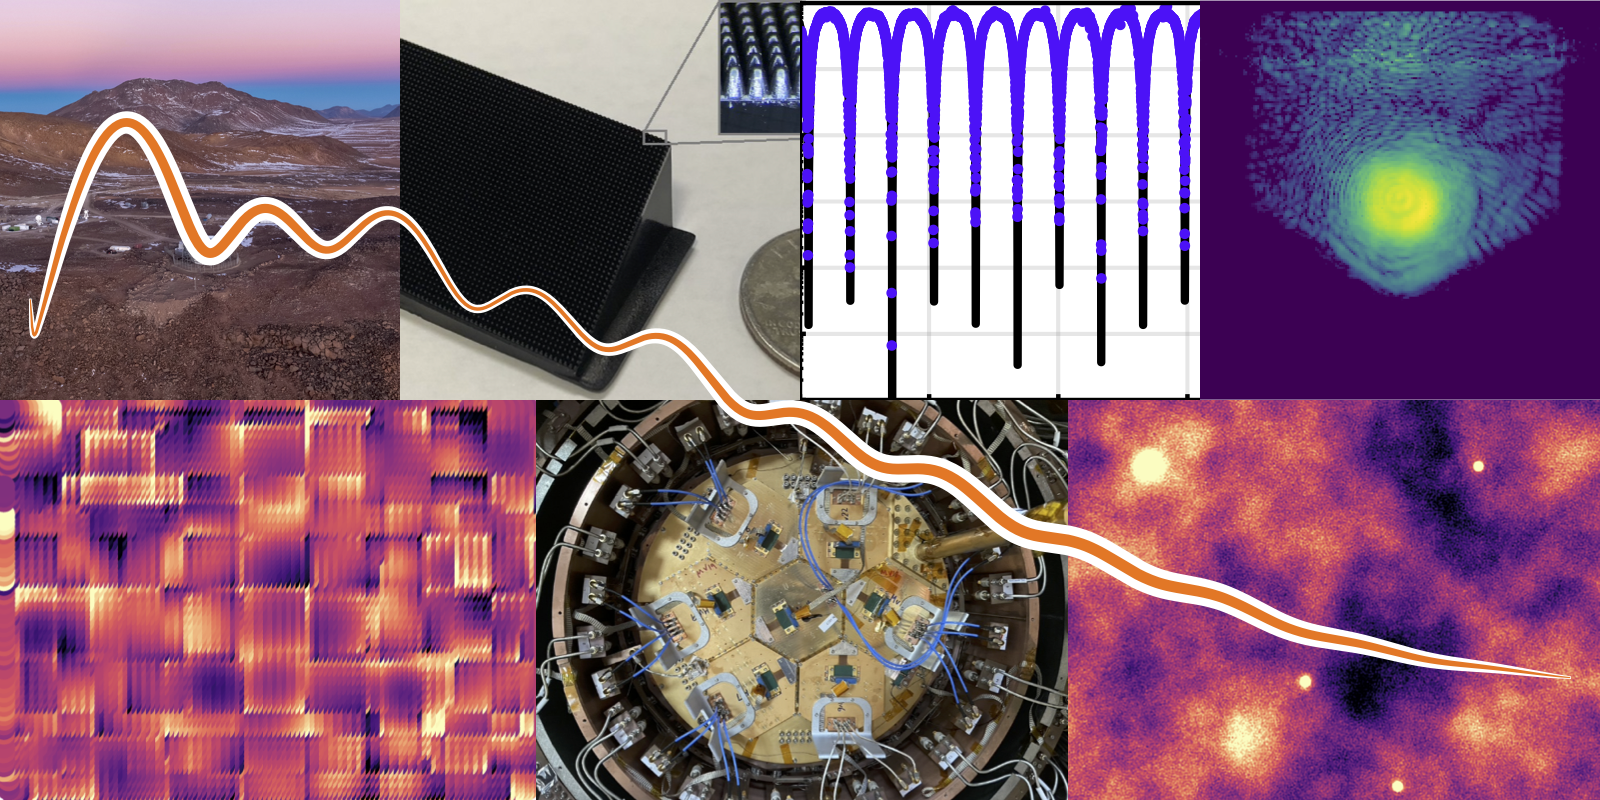
\includegraphics[width = \textwidth]{Figures/conclusion.png}
    \label{fig:finalfigure}
\end{figure}
Experimental cosmology is in an era of precision instrumentation.  Such precision instrumentation requires understanding optical components in the telescope, careful characterization of its performance, and detailed analysis of its optical performance.  In this work, I have presented several advances in instrumentation and optics which will advance our understanding of the universe.  I have also presented novel methods for characterizing the instruments to further improve systematics. 

\section{Optical Characterization of Materials}
Understanding the optical properties of the materials within the telescope is crucial for predicting its optical performance.  This becomes even more critical as detectors increase in sensitivity; optical systematics need to be tightly constrained.
In this work, I presented the characterization of a variety of optical components for ground-based cosmological experiments.  

\subsection{Meta-material Absorbers for Stray Light}
As detector sensitivity improves, systematics must be mitigated. For example, stray light within an optics tube results in loading onto the detectors, degrading the signal-to-noise of the camera.  To control and mitigate unwanted scattering within the optical system, we develop meta-material absorbers which stop the scattering at the front of the telescope prior to entering deeper into the optics tube.  
 
As presented in Chapter~\ref{ch:mma}, we use the holography receiver to characterize the meta-material absorbers in the mid-frequency band.  We measure the reflectivity and scattering properties of the meta-material absorber, and compare its performance to alternative absorbers used in experimental cosmology.  We find he integrated scattering power is less than 1\% with the angle of incidence  $\leq45\deg$.  \textcolor{red}{Sentence about the significance of this finding...}


\subsection{Silicon Lenses}
Silicon is an optimal material for re-imaging the millimeter-wave photons onto detectors.  Its index of refraction provides fast re-imaging of the beam onto the detectors with low loss of signal.  The specific index of refraction informs the optical design of the telescope, and thus it is crucial to know the exact loss and optical properties of the lenses during the optical design.  The loss tangent is critical to constrain, as it dictates the loss of power as signal propagates through a medium.

Chapter~\ref{ch:si} reports the measured reflectivity of two silicon samples for potential use in cosmology experiments, and here are studied using a holography imaging setup.  From the reflectivity, we determine the loss-tangent of both samples, and find the "intrinsic" silicon has a lower loss-tangent than the neutron-doped silicon across the mid-frequency band (75-160\,GHz), therefore making it a better material for lenses in experimental cosmology.

\section{Characterization of the Large Aperture Telescope Receiver Tester for Simons Observatory}
Integrating and testing the optical performance of a telescope prior to deployment is novel; it is common to characterize the beam of a telescope at the site.  However, once at the site, it is nearly impossible to alter the hardware and probe its functionality.  In Chapter~\ref{ch:ot_holo}, we present the characterization of the Simons Observatory Large Aperture Telescope Receiver with radio holography.

From this optical characterization, we found a source of scattering which, when removed, improved efficiency in the mid-frequency band by roughly 5\%.  Characterizing the fully integrated optical system allowed for multiple tests and the careful discovery of additional sources of scattering prior to deployment.  We also determined the on-sky beam prior to deployment by propagating the near-field measured beams through the LAT and into the far-field, verifying the on-sky beam size was within SO's requirement.  \textcolor{red}{Sentence about the significance of this finding...}

\section{Characterization of the Small Aperture Telescope for Simons Observatory}
Following the characterization of the LAT optical system, we present preliminary results of the SAT optical system measured with the same radio holography receiver (Chapter~\ref{ch:sat_holo}).  Though results are preliminary, we determine the on-sky beam to be within 10\% of the expected beam size in the mid-frequency band.  This further demonstrates the applicability of radio-holography system to other optical systems prior to deployment.  

\section{Wavefront Optimization with Radio Holography and Machine Learning}

To enable large aperture cosmology experiments, it is common to use large reflector mirrors which are made up of many panels.  Such reflectors can create wavefront errors due to the Ruze principle.  In Chapter~\ref{ch:holosim}, we presented the SO dual reflector optical system (Large Aperture Telescope) and a method of measuring the panel offsets using radio holography paired with machine learning.  This approach can yield $<5\,\mu$m alignment errors, the requirement for SO science goals.

\section{Point Source Stacking for AdvACT}
